\documentclass[10pt]{amsart}
\usepackage{amsmath}
\usepackage{amsthm}
\usepackage{tikz}
\usepackage{booktabs}
\usetikzlibrary{shapes.geometric, arrows}


\usepackage{minted}


\newcommand{\R}{\mathbb{R}}
\newcommand{\C}{\mathcal{C}}
\renewcommand{\u}{\mathbf{u}}
\renewcommand{\v}{\mathbf{v}}
\newcommand{\w}{\mathbf{w}}
\newcommand{\x}{\mathbf{x}}
\newcommand{\y}{\mathbf{y}}
\renewcommand{\b}{\mathbf{b}}
\newcommand{\e}{\mathbf{e}}
\newcommand{\s}{\mathbf{s}}


\newcommand{\A}{\mathbf{A}}
\newcommand{\B}{\mathbf{B}}
\newcommand{\W}{\mathbf{W}}

\newtheorem{theorem}{Theorem}[section]
\newtheorem{proposition}[theorem]{Proposition}
\newtheorem{lemma}[theorem]{Lemma}
\newtheorem{corollary}[theorem]{Corollary}


\theoremstyle{definition}
\newtheorem{definition}[theorem]{Definition}
\newtheorem{example}[theorem]{Example}


\begin{document}
\title{Recurrent Neural Networks}
\author{Jean-Martin Albert}
\date{\today}
\maketitle


 \section{Introduction}

Throughout this handout, we use bold face lower case letters to represent vectors, and bold face capital letters to represent matrices.  Most of the time, we will blur the dustinction between matrices and vectors, except when it makes the exposition clearer.

 Let $f:\R^n\to \R^m$ be a function, and consider a class $\C$ of functions $g: \R^n\to \R^m$, which we assume to be parametrized by $\R^\ell$, in the sense that there is a function $F(\x,\w):\R^n\times \R^\ell\to\R^n$ such that $\C=\{\x\mapsto F(\x,\w):\w\in\R^n\}$.  The generic problem of machine learning is to find a vector $\w\in\R^{\ell}$ such that $D(f(\x), F(\x, \w))$ is as small as possible, where $D$ represents a notion of distance between functions, for example, $$D(f(\x), F(\x, \w)) = \min\{\|f(\x)-F(\x, \w)\|:\x\in\R^n\}$$ Note that since the minimum is computed over all possible vlues of $\x$, the value of $D$ in te equation above depends on $\w$.  Define $$\ell(\w)=D(f(\x), F(\x, \w))$$ Given the definition of $D$, we see that $\ell(\x)\geq 0$, and therefore $\ell$ has a global minimum (which is not necessarily unique). In general, the global minimum of $\ell$ is not attained, in the sense that if $\epsilon=\min\{\ell(\w):\x\in\R^n\}$, then there does not necessarily exist a value $\w_0\in\R^\ell$ such that $\epsilon=\ell(\w_0)$.  However, it can be approximated, that is to say there is a sequence $\w_i$ such that $\ell(\w_i)\to\epsilon$ as $i\to\infty$.  We may not be able to achieve the minimum with a specific value of $\w$, but we can get as close to it as we want: for every $\varepsilon>0$, there is some natural number $N_\varepsilon>0$ such that $\|\epsilon-\ell(\w_i)\|<\varepsilon$ for every $i>N_\varepsilon$. Since we can choose $\varepsilon$ to be as small as we want, if we choose it to be smaller than the smallest number which can be represented with a {\tt float32} (say), then from the point of view of any program, $\ell(\w_i)=\epsilon$ when $i>N_\varepsilon$.

 The function $\ell$ we defined above is called a {\em loss function}.  There are many functions which are suitable for $\ell$.  In fact, $\ell$ does not need to represent a distance at all. In order to draw a meaningful conclusion from the minimum value of $\ell$, all we need to know is that $\ell(\w)=0$ implies $f(\x)=F(\x,\w)$ for every $\x$, or at the very least $\|f(\x)-F(\x,\w)\|\leq\varepsilon$ for arbitrary $\varepsilon$.  In every neural network we define, we specify a class of functions $F(\x, \w)$, and a definition for $\ell(\w)$ based on $F$. In tensorflow, the function we are trying to approximate is given in the form of a relation $f(\x)=\y$. We provide {\em placeholders} for the values of $\x$ and $\y$.  The function $F(\x,\w)$ is defined by a computation graph.  For example, here is a linear regression, in which we try to approximate a function $f:\R^{10}\to\R^{15}$ using a function of the form $F(\x, \W\b)=\W\x+\b$. Here $\W$ is an $15\times 10$ matrix, and $\b\in\R^{15}$

 \begin{minted}{python}
 x = tf.placeholder(shape=[None, 10])
 y = tf.placeholder(shape=[None, 15])
 W = tf.Variable(shape=[None, 10, 15])
 b = tf.Variable(shape=[None, 15])
 F = tf.matmul(x, W) + b
 loss = tf.mean_square_error(y, F)
 \end{minted}


We are mainly interested in classification problems, or more generally problems which can be expressed as classification problems. Let $A$ and $B$ be finite sets, and let $f:A\to B$ be any function.  In order to use neural networks, which represent functions between topological vector spaces, to represent  function between ordinary sets, we must first translate the sets $A$ and $B$ into vector spaces.  The most straightforward (and freest) way to interpret a set $A$ as a vector space is to use $A$ as the basis for a vector space.  Write $A=\{a_1,...,a_n\}$, and let $\{\e_1,...,\e_n\}$ represent the standard basis for $\R^n$.  Let $e:A\to\R^n$ be defined by $e(a_i)=\e_i$.  Similarly, we can write $B=\{b_1,...,b_m\}$, and define $e:B\to \R^m$ by $e(b_i)=\e_i$.  This specific function is called {\em one-hot encoding}, and is present in tensorflow as tf.onehot.  Since we are mapping a finite set to an infinte set, the function $e$ has no inverse, but it has a "pseudo-inverse" given by the {\em argmax()} function defined by $argmax(\v)=i$ where $i$ is smallest such that $v_i\geq v_j$ for every $j\not=i$. In other words, $argmax$ computes the index of the largest component of a vector.

Given $\v\in\R^m$ is the output of $F(\x,\w)$, then if $\v$ has the property that $\sum v_i=1$, and $v_i\geq 0$ for every $i$, then we can interpret $\v$ as a probability distribution, where each component $v_i$ represents the probability that $\v=\e_i$.  The code, in tensorflow, which approximates a function $A\to B$ can be written as:

\begin{minted}{python}
x_in = tf.placeholder(shape=[None, 1])
x = tf.one_hot(x_in, 10)
y_in = tf.placeholder(shape=[None, 1])
y = tf.one_hot(y_in, 15)
W = tf.Variable(shape=[None, 10, 15])
b = tf.Variable(shape=[None, 15])
F = tf.softmax(tf.matmul(x, W) + b)
loss = tf.cross_entropy(y, F)
\end{minted}

The softmax function in the penultimate line is defined by $\sigma(\v) = \w$  where $$w_i= \frac{e^{v_i}}{\sum e^{v_j}}$$ Note that $\sum w_j=1$, which means that the output of the softmax function can be interpreted as a probability distribution.  This makes it a popular choice for classification problems with many classes.  If the target space is $\R^2$, then this reduces to a binomial distribution.  The cross-entropy function in the last line is defined by $C(\v, \w) = -\sum(v_i\log(w_i))$.  Intuitively, $C$ measures the number of vector components that are necessary to differentiate between the distribution $\v$ and the distribution $\w$.  Therefore, the optimal value for $C$ to have is $N$: measuring any bit should allow us to differentiate between $\v$ and $\w$.  Note that $C(\v, \w)=1$ if and only if $\log C(\v, \w)=0$, so that the logarithm of the cross entropy function is a candidate for a distance function. The vector $\w$ here should be the output of the model, whereas $\v$ should be the true value.  By definition, $w_i= \frac{e^{v_i}}{\sum e^{v_j}}$, so that $\log(w_i) = \log e^{w_i} - \log(\sum e^{v_j}) = w_i - \log(\sum e^{v_j})$. By definition again, $v_i=1$ and $v_j=0$ if $i\not=j$. Therefore, $C(\v, \w) = w_i + \log(\sum e^{w_j})$


\section{Dealing with sequences}

\subsection{Basic theory} Classical neural networks are great for classification problems involving either fixed (finite) sets $f:A\to B$, where $A$ represents the set to be classified, and $B$ is the set of labels, or functions $f:\R^n\to B$. An example of the latter is image classification, since an $n\times m$ image can be directly represented as a vector in $\R^{\ell mn}$. In many cases, however, the data to be classified is better represented as a (finite) sequence.  For example, sentences are sequences of words, words are sequences of letters, movies are sequences of images, and sound files are sequences of amplitudes.  It is possible to deal with sequences with ordinary neural networks, but we run into difficulties when we try to model dependency between different elements of a sequence.  Let $A$ be a finite set. A finite sequence of elements of $A$ is a tuple $(a_1,...,a_n)$, where $a_i\in A$ for every $i$.  Here the number $n$ is allowed to change.  The set of all finite sequences of elements of $A$ is denoted $A^*$.  From the definition we just gave, we have $A^*=\bigcup_{n\geq 0} A^n$, which is a good enough definition for our purpose.  If we are given two finite sets $A$ and $B$, there are many situations we can consider if we also have access to $A^*$ and $B^*$.
\begin{enumerate}
  \item A function $f:A\to B^*$, which given an element of $A$ outputs a sequence of elements of $B$.  This is called a {\em one-to-many} function. We use this architecture in a sequence sorting neural network. The Tweet2Vec autoencoder also uses a one-to-many neural network.
  \item A function $f:A^*\to B$, which is given a sequence of elments of $A$ and produces a single element of $B$.  This is called a {\em many-to-one} function.  A good example of sich a function is the Buzzometer sentiment analysis tool which assigns a single sentiment value to messages which can vary in length.
  \item A function $f:A^*\to B^*$ which is given a seuqence of elements of $A$< and outputs a sequence of elements of $B$.  This is called a {\em many-to-many} function.  As an example of such a function we will show the implementation of a simple text generator.  Translation, video captioning, part-of-speech tagging and speech recognition are all examples of many-to-many functions.
\end{enumerate}

We can of course define functions $A\to B^*$, $A^*\to B$ and $A^*\to B^*$ directly (they are just sets, after all), but it is more interesting and instructive to make use of the structure of $A^*$ and $B^*$ as sets of sequences of $A$ and $B$, and see how one can use a function (or class of functions) $A\to B$ to define a function $A^*\to B^*$. In particular, we will me making use of the iterative nature of the construction $A^*$ and $B^*$. Here is the simplest example: if $A=B$, and $f:A\to A$ is a function, then we can iterate $f$: $f^0(a)=a$ for every $a\in A$, and $f^{n+1}(a) = f(f^n(a))$. We terminate the iteration at the first value of $n$ for which $f^n(a)=f^{n-1}(a)$ (note that there is no guarantee that this will ever happen). This gives a function $f:A\to A^\omega$.

We describe a more general situation. Let $S$ be a (finite) set of {\em states} with a distinguished element $\perp\in S$, and consider a function $f:A\times S\to B\times S$. Let $a_1,...,a_n$ be a finite sequence of elements of $A$.  We define two sequences $b_1,...,b_n$ and $s_1,...,s_n$ of elements of $B$ and $S$ respectively as follows.  We first define $b_1, s_1 = f(a_1, \perp)$.  Suppose that we have defined the elements $b_1,...,b_n$ and $s_1,...,s_n$.  We define $b_{n+1}$ and $s_{n+1}$ via $b_{n+1}, s_{n+1} = f(a_{n+1}, s_n)$.  We define $f^*(a_1...a_n)=b_1...b_n$, with $b_1,...,b_n$ defined as above.  This is a function $f^*:A^*\to B^*$, and it has the property that the length of the output sequence is the same as that of the input sequence.  An interesting special case of this is when $S=B$. In this case, we can have $f:A\times B\to B$. We can define b_1 = f(a_1, \perp)$, and $b_{n+1}=f(a_{n+1}, b_n)$. This is in fact the main type of function we use in our examples later. Note that this is a state machine, close to a deterministic finite automaton, except that here the state space $S$ is allowed to be infinite.

We use the exact same method to define a many-to-one function. If $f:A\times S\to B\times S$ is a function, and  $a_1,...,a_n$, $b_1,...,b_n$ and $s_1,...,s_n$ are defined as above, then we define $f^*(a_1,...,a_n)=b_n$.  In other words, we discard all elements of $B$ produced during the iteration, and keep only the last one.

Finally, we tackle the case of a one-to-many function. Again we let $f:A\times S\to B\times S$ be any function. We define sequences $b_1,...,b_i,...$ and $s_1,...,s_i,...$ as follows. $b_1,s_1=f(a,\perp)$, and for every $n$, $b_{n+1}, s_{n+1}=f(a, s_n)$. In other words, we keep iterating $f$, feeding $a$ as input at every step. An imoprtant variant of this is when $a$ itself has a distinguished element $\perp_A$, in which case, after feeding $a$ as an input to $f$ in the first iteration, we subsequently feed it $\perp_A$, and get $b_{n+1}, s_{n+1}=f(\perp_A, s_n)$.  We stop the iteration whenever $s_n=\perp$ (or any other predetermined element of $S$). Note that this may never happen, i.e. the sequence $b_n$ may go on forever. In fact, there is no way to give a general pattern of definition for $f:A\times S\to B\times S$ which will guarantee that $f^*(a)$ is finite for every $a$.


\subsection{Recurrent networks}

In general, a recurrent neural network is just a presceiption for a class of functions of the form $f:\R^n\times \R^\ell\times\R^m\to \R^m\times \R^\ell$, where $\R^m$ is the space of parameters. The set $\{0,1\}^*$ of all finite sequences of $0$'s and $1$'s is countable, and $\R^\ell$, being a real vector space,
is uncountable.  Therefore, we can encode every element $w\in\{0,1\}^*$ as a vector in $S$.  Informally,
$\R^\ell$ is enough to encode any finite state space, and every possible value for the content of the tape of a
Turing machine. We get:

\begin{theorem}
Recurrent neural networks are Turing-complete.
\end{theorem}

This explains why recurrent neural networks seem to be able to produce results that other networks can't. Training a recurrent network is the same as producing a Turing machine.  A common way to represent a recurrent node is to use a box, the inside of which represent the definition of $f$.  The vertical arrows represent the input and onput of the node, and the horisontal arrows represent the input and output state of the node.

\begin{center}
  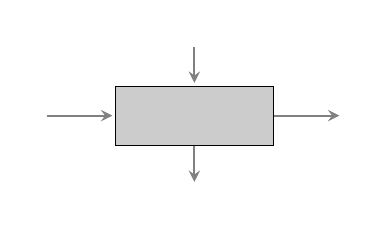
\begin{tikzpicture}[shorten >=1pt,->,draw=black!50, node distance=1cm]
    \tikzstyle{arrow} = [thick,->,>=stealth]
    \tikzstyle{startstop} = [rectangle, minimum width=2cm, minimum height=.75cm, text centered, draw=black, fill=black!20]
    \node (input) [] at (0cm,1cm) {};
    \node (output) [] at (0cm,-1cm) {};
    \node (s-input) [] at (-2cm,0cm) {};
    \node (s-output) [] at (2cm,0cm) {};
    \path[] node[startstop] (N) at (0cm,0cm) {};
    \draw [arrow] (input) -- (N);
    \draw [arrow] (s-input) -- (N);
    \draw [arrow] (N) -- (output);
    \draw [arrow] (N) -- (s-output);
\end{tikzpicture}
\end{center}

Just like any regular neural network layer, recurrent nodes can be composed.  The composition of two recurrent nodes is done by feeding the output of one node into the input of the other, and concatenating their state space.  Formally, if $f:\R^n\times \R^\ell\times\to \R^m\times \R^\ell$ and $g:\R^n\times \R^\ell\times\to \R^m\times \R^\ell$ are two recurrent nodes, then we have the node $(f;g):\R^m\times\R^\ell\times\R^L\to\R^k\times\R^\ell\times\R^L$ defined by $(f;g)(\x, \s_1, \s_2) = (\y, \s'_1, \s'_2)$ where $f(\x, \s_1) = \x', \s'_1$ and $g(\x', \s_2) = \y, \s'_2$. Graphically, we can represent this by stacking the boxes representing $f$ and $g$ on top of one another:

\begin{center}
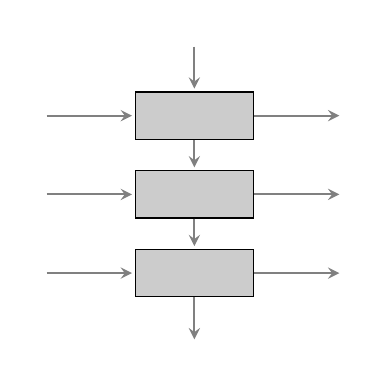
\begin{tikzpicture}[shorten >=1pt,->,draw=black!50, node distance=1cm]
    \tikzstyle{arrow} = [thick,->,>=stealth]
    \tikzstyle{startstop} = [rectangle, minimum width=1.5cm, minimum height=.6cm, text centered, draw=black, fill=black!20]
    \node (input) [] at (0cm,1cm) {};
    \node (output) [] at (0cm,-3cm) {};
    \node (s-input-A) [] at (-2cm,0cm) {};
    \node (s-output-A) [] at (2cm,0cm) {};
    \node (s-input-B) [] at (-2cm,-1cm) {};
    \node (s-output-B) [] at (2cm,-1cm) {};
    \node (s-input-C) [] at (-2cm,-2cm) {};
    \node (s-output-C) [] at (2cm,-2cm) {};
    \path[] node[startstop] (A) at (0cm,0cm) {};
    \path[] node[startstop] (B) at (0cm,-1cm) {};
    \path[] node[startstop] (C) at (0cm,-2cm) {};
    \draw [arrow] (input) -- (A);
    \draw [arrow] (s-input-A) -- (A);
    \draw [arrow] (s-input-B) -- (B);
    \draw [arrow] (s-input-C) -- (C);
    \draw [arrow] (A) -- (s-output-A);
    \draw [arrow] (B) -- (s-output-B);
    \draw [arrow] (C) -- (s-output-C);
    \draw [arrow] (A) -- (B);
    \draw [arrow] (B) -- (C);
    \draw [arrow] (C) -- (output);
\end{tikzpicture}
\end{center}

The whole stack can then be seen as one single recurrent node.

\section{Training}

\subsection{The standard version} In general, in order to minimize a function $f(w)$ of one variable, we make use of the fact that the extreme values of $f$ all have $f'(x)=0$.  If $f$ is a function of two or more variables, then if $x$ is such that $f(x)$ is a local max, or minimum, then all partial derivatives $\frac{\partial f}{\partial w_i}(x)=0$.  If $f:\R^n\to\R$ is a function, then the {\em gradient} of $f$ is the vector $\nabla f(x) = \left(\frac{\partial f}{\partial w_1}(x),...,\frac{\partial f}{\partial w_n}(x)\right)$. One interesting property of $\nabla f(x)$ is that, as a vector, it ``points'' in the direction in which $f$ decreases the most.  That is to say, there is a good chance that $f(x-\alpha\nabla f(x))\leq f(x)$. The chance is better the smaller $\alpha$ is.  We see that if we iterate that process, we get a sequence $x_1,...,x_n,...$ such that $f(x_{i+1})\leq f(x_i)$ for every $i$.  Since $m\leq f(x_i)\leq f(x_0)$ for every $i$, we get a bounded decreasing sequence of real number, which converges.

Caveat: this ideal situation doesn't allways happen.

This iterative process is {\em (Stocastic) gradient descent}.

Suppose $f$ is a complsition of two functions, and that we can write $f(x,w)= g(h(x, w_1), w_2)$.
Then we can write $\nabla_w f(x, w)=\nabla g(h(x, w_1), w_2)\cdot \nabla h(x, w_1)$. Each level
of composition corresponds to a layer of neural network.  The chain rule transforms function composition
into a product. If a network becomes deep, then the derivative of the loss function becomes a long
product.  When gradients become small in norm (like they do when we approach a min), then the gradient
becomes very close to $0$, and the update rule for gradient descent stops changing the weights.

This is the vanishing gradient problem for very deep networks, and makes convergence slow.


\subsection{Backward Propagation Through Time}
How do we train recurrent neural networks? we can use back propagation, just like a regular neural network. Heuristically, we unroll the recurrent network ``infinitely'' many times, until it looks like an ordinary very deep neural network.  In practice, since computers only have a finite amount of resources, we only unroll the network a large but finite number of times, and treat it like an ordinary neural network.

\begin{tikzpicture}[shorten >=1pt,->,draw=black!50, node distance=1cm]
    \tikzstyle{arrow} = [thick,->,>=stealth]
    \tikzstyle{startstop} = [rectangle, minimum width=1.5cm, minimum height=.6cm, text centered, draw=black, fill=black!20]
    \node (input) [] at (0cm,1cm) {};
    \node (output) [] at (0cm,-1cm) {};
    \node (s-input-A) [] at (-2cm,0cm) {};
    \node (s-output-A) [] at (10cm,0cm) {};
    %\node (s-input-B) [] at (-2cm,-1cm) {};
    %\node (s-output-B) [] at (10cm,-1cm) {};
    %\node (s-input-C) [] at (-2cm,-2cm) {};
    %\node (s-output-C) [] at (10cm,-2cm) {};
    \path[] node[startstop] (A-0) at (0cm,0cm) {};
    %\path[] node[startstop] (B-0) at (0cm,-1cm) {};
    %\path[] node[startstop] (C-0) at (0cm,-2cm) {};
    \draw [arrow] (input) -- (A);
    \draw [arrow] (s-input-A) -- (A-0);
    %\draw [arrow] (s-input-B) -- (B-0);
    %\draw [arrow] (s-input-C) -- (C-0);
    %\draw [arrow] (A) -- (B);
    %\draw [arrow] (B) -- (C);
    \draw [arrow] (A) -- (output);

     \foreach \i/\j in {1/0,2/1,3/2,4/3}
     {
       \node (input-\i) [] at (2*\i cm,1cm) {};
       \node (output-\i) [] at (2*\i cm,-1cm) {};
       \path[] node[startstop] (A-\i) at (2*\i cm,0cm) {};
    %   \path[] node[startstop] (B-\i) at (2*\i cm,-1cm) {};
  %     \path[] node[startstop] (C-\i) at (2*\i cm,-2cm) {};
  %     \draw [arrow] (A-\i) -- (B-\i);
%       \draw [arrow] (B-\i) -- (C-\i);
       \draw [arrow] (input-\i) -- (A-\i);
       \draw [arrow] (A-\j) -- (A-\i);
%       \draw [arrow] (B-\j) -- (B-\i);
%       \draw [arrow] (C-\j) -- (C-\i);
       \draw [arrow] (A-\i) -- (output-\i);
     }
     \draw [arrow] (A-4) -- (s-output-A);
     %\draw [arrow] (B-4) -- (s-output-B);
     %\draw [arrow] (C-4) -- (s-output-C);

\end{tikzpicture}




\section{Types of Recurrent Cells}


In this section we descripbe three of the main types of recurrent cells currently in use.  They are the basic recurrent cell, which is a straightforward implementation of a function $f:\R^n\times\R^\ell\to\R^\ell$, then long short term memory cell (LSTM), which is more suitable to model long term dependencies in sequences, and the gated recurrent unit cell, which is a simplification of the LSTM cell, but which performs almost equally well at long term dependencies. We give a formal definition of each oc these cells along with a na\"ive implementation in {\tt tensorflow}. The implementation we provide is only expositional though, and would not work out of the box in an actual production model.
%There are three main types of recurrent cells which are used to build recurrent neural networks.  Let us describe them, and give some of their basic properties, along with a na\"ive implementation in tensorflow.

\subsection{Basic Recurrent Cell} We begin with the most basic of recurrent cell. Abstractly, a function $f:U\times S\to V\times S$ can be defined using two functions $u:\R^n\times \R^\ell\to \R^n$ and $v:\R^n\times\R^\ell \to \R^\ell$. We se ethe former function as providing the output, and the latter function as a state updating function.  The most common definition for $u$ and $v$ for basic recurrent cells is as follows: $u(x, s) = f(A_ux+B_us)$, where $A$ nad $B$ are matrices, and $f$ is a non-linear function, and $v(x, s) = \tanh(A_vx+B_vs)$. Te parameters in this definition are $A_u$, $B_u$, $A_v$ and $B_v$. In tehsorflow, the code looks like:

\begin{minted}{python}
def basic_rnn_cell(input_tensor, state_tensor, output_dimension):
  input_dimension = input_tensor.get_shape()[1]
  state_dimension = input_tensor.get_shape()[1]
  A_u = tf.Variable(shape=[input_dimension, output_dimension])
  B_u = tf.Variable(shape=[state_dimension, output_dimension])
  A_v = tf.Variable(shape=[input_dimension, state_dimension])
  B_v = tf.Variable(shape=[state_dimension, state_dimension])
  output_tensor = tf.relu(tf.matmul(input_tensor, A_u) + \
                            tf.matmul(state_tensor, B_u))
  new_state_tensor = tf.tanh(tf.matmul(input_tensor, A_v) + \
                                  tf.matmul(state_tensor, B_v))
  return output_tensor, new_state_tensor
\end{minted}

A variant of this cell uses the output as a state vector, thus computing every step as a function of the cirrent ouput, and the previous output.


\subsection{Long Short-term Memory Cell} There are a few problems with the architecture described above.  First, it suffers greatly from the vanishing gradient problem, since there is no way to prevent gradients from becoming very small.  Secondly, simple recurrent networks have a hard time remembering facts about the input sequence.  To remedy this situation, long short-term memory cells were introduced.  The overall structure of an LSTM cell is almost the same as the basic RNN cell. This time we take the previous output into account, which gives the structure as $f:\R^n\times \R^m\times \R^{\ell}\to \R^m\times \R^{\ell}$ which can be divided as two function $u:\R^{n}\times\R^m\times \R^{\ell}\to \R^m$ and $v:\R^n\times \R^m\times\R^{\ell}\to \R^{\ell}$. To define the functione $u$ and $v$, we use auxiliary functions $F$, $I$, and $O$ defined as follows
\begin{eqnarray*}
  F(x, y) &=& \sigma(A_Fx + B_Fy + b_F)\\
  I(x, y) &=& \sigma(A_Ix + B_Iy + b_I)\\
  O(x, y) &=& \sigma(A_Ox + B_Oy + b_O)\\
  S(x, y) &=& \sigma(A_Ox + B_Oy + b_O)\\
\end{eqnarray*}
The state update is given by $v(x, y, s) = F(x, y)\circ s + I(x, y)\circ \sigma_v(A_vx + B_vy + b_v)$, where $\circ$ denotes pointwise multiplication of vectors, and finally, the output can be defined as $u(x, y, s)=O(x, y)\circ \sigma_u(v(x, y, s))$.

\begin{minted}{python}
def lstm_gate(input_tensor, previous_output, port_op):
  A = tf.Variable(shape=[N, L])
  B = tf.Variable(shape=[L, L])
  b = tf.Variable(shape=[L, L])
  x = tf.matmul(input_tensor, A)+ tf.matmul(previous_output, B) + b
  return post_op(x)

def lstm_cell(input_tensor, output, state):
  F = lstm_gate(input_tensor, output, tf.sigmoid)
  I = lstm_gate(input_tensor, output, tf.sigmoid)
  O = lstm_gate(input_tensor, output, tf.sigmoid)
  S = lstm_gate(input_tensorm output, tf.tanh)
  new_state = tf.mul(output, F) + tf.mul(I, S)
  output = tf.mul(O, tf.tanh(new_state))
  return output, new_state
\end{minted}



%The function $u$ is defined by $u(x, o, s)=o()$



%: a function $f:\R^n\times \R^{\ell}\to \R^m\times \R^{\ell}$, which can be divided as two function $u:\R^{n}\times \R^{\ell}\to \R^m$ and $v:\R^n\times\R^{\ell}\to \R^{\ell_1}$.  We can se the function $u$, like before, as providing the output. The function $v$ can be seen as the state update function.  The function $u$ is defined by $u(x, s)=\sigma(A_U x+)$

% above, but the state space is further divided as $\R^\ell=\R^{\ell_1}\times\R^{\ell_2}$, which gives the cell the structure of a function $f:\R^n\times \R^{\ell_1}\times\R^{\ell_2}\to \R^m\times \R^{\ell_1}\times\R^{\ell_2}$, which can be divided as three function $u:\R^{n}\times \R^{\ell_1}\times\R^{\ell_2}\to \R^m$,  $v:\R^n\times\R^{\ell_1}\times\R^{\ell_2} \to \R^{\ell_1}$ and $w:\R^n\times\R^{\ell_1}\times\R^{\ell_2} \to \R^{\ell_2}$.  We can se the function $u$, like before, as providing the output. The function $v$ can be seen as the state update function, and the function $w$ controls a memory tape.

\subsection{Gated Recurrent Unit Cell} A common variant of the long short term memory cell is the {\em gated recurrent unit cell}, more commonly known as GRU cells.  The philosophy behind their design is similar to the long short term memory. Once again, each step of the computation takes into account a state vector and the output of the previous iteration. GRU's are functions  $f:\R^n\times \R^m\times \R^{\ell}\to \R^m\times \R^{\ell}$,  which can be divided as two function $u:\R^{n}\times\R^m\times \R^{\ell}\to \R^m$ and $v:\R^n\times \R^m\times\R^{\ell}\to \R^{\ell}$. To define the functione $u$ and $v$, we use auxiliary functions $U$ and  $R$ defined as follows
\begin{eqnarray*}
  U(x, y) &=& \sigma(A_Ux + B_Uy + b_U)\\
  R(x, y) &=& \sigma(A_Rx + B_Ry + b_R)\\
\end{eqnarray*}
The state update is given by $v(x, y, s) = U(x, y)\circ s + (1-s)\circ \sigma_h(A_v x + B_v(R(x, y)\circ y) + b_v)$.

\begin{minted}{python}
def gru_gate(input_tensor, previous_output, port_op):
  A = tf.Variable(shape=[N, L])
  B = tf.Variable(shape=[L, L])
  b = tf.Variable(shape=[L, L])
  x = tf.matmul(input_tensor, A)+ tf.matmul(previous_output, B) + b
  return post_op(x)

def gru_cell(input_tensor, output, state):
  U = gru_gate(input_tensor, output, tf.sigmoid)
  R = gru_gate(input_tensor, output, tf.sigmoid)
  O = gru_gate(input, tf.mul(R, output))
  return tf.mul(R, output) + tf.mul((1-R)O)
\end{minted}



%$$
%$$
%
%I(x, y)\circ \sigma_v(A_vx + B_vy + b_v)$, where $\circ$ denotes pointwise multiplication of vectors, and finally, the output can be defined as $u(x, y, s)=O(x, y)\circ \sigma_u(v(x, y, s))$.


\section{Examples}

\subsection{Many-to-One}

The Buzzometer sentiment analysis tool uses a bi-directional GRU model, in which the output a 4-layer
bidirectional recurrent network is fed into a two-layer fully connected network which separates the input into
four classes, corresponding to neutral, positive, negative and irrelevant messages. The only non-linearities
 in the network are inside the GRU cells.  Graphically, the network can be represented as:

%(GRAPHICAL REPRESENTATION OF NETWORK)
\begin{tikzpicture}[shorten >=1pt,->,draw=black!50, node distance=1cm]
    \tikzstyle{arrow} = [thick,->,>=stealth]
    \tikzstyle{startstop} = [rectangle, minimum width=1.5cm, minimum height=.6cm, text centered, draw=black, fill=black!20]
    \node (input) [] at (0cm,1cm) {};
    \node (output) [] at (0cm,-3cm) {};
    \node (s-input-A) [] at (-2cm,0cm) {};
    \node (s-output-A) [] at (10cm,0cm) {};
    \node (s-input-B) [] at (-2cm,-1cm) {};
    \node (s-output-B) [] at (10cm,-1cm) {};
    \node (s-input-C) [] at (-2cm,-2cm) {};
    \node (s-output-C) [] at (10cm,-2cm) {};
    \path[] node[startstop] (A-0) at (0cm,0cm) {};
    \path[] node[startstop] (B-0) at (0cm,-1cm) {};
    \path[] node[startstop] (C-0) at (0cm,-2cm) {};
    \draw [arrow] (input) -- (A);
    \draw [arrow] (s-input-A) -- (A-0);
    \draw [arrow] (s-input-B) -- (B-0);
    \draw [arrow] (s-input-C) -- (C-0);
    \draw [arrow] (A) -- (B);
    \draw [arrow] (B) -- (C);
    \draw [arrow] (C) -- (output);

     \foreach \i/\j in {1/0,2/1,3/2,4/3}
     {
       \node (input-\i) [] at (2*\i cm,1cm) {};
       \node (output-\i) [] at (2*\i cm,-3cm) {};
       \path[] node[startstop] (A-\i) at (2*\i cm,0cm) {};
       \path[] node[startstop] (B-\i) at (2*\i cm,-1cm) {};
       \path[] node[startstop] (C-\i) at (2*\i cm,-2cm) {};
       \draw [arrow] (A-\i) -- (B-\i);
       \draw [arrow] (B-\i) -- (C-\i);
       \draw [arrow] (input-\i) -- (A-\i);
       \draw [arrow] (A-\j) -- (A-\i);
       \draw [arrow] (B-\j) -- (B-\i);
       \draw [arrow] (C-\j) -- (C-\i);
       \draw [arrow] (C-\i) -- (output-\i);
     }
     \draw [arrow] (A-4) -- (s-output-A);
     \draw [arrow] (B-4) -- (s-output-B);
     \draw [arrow] (C-4) -- (s-output-C);

\end{tikzpicture}


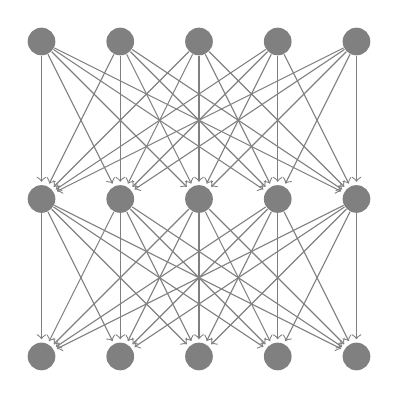
\begin{tikzpicture}[shorten >=1pt,->,draw=black!50, node distance=1cm]
    \tikzstyle{every pin edge}=[<-,shorten <=1pt]
    \tikzstyle{neuron}=[circle,fill=black!50,minimum size=10pt,inner sep=0pt]

    % Draw the hidden layer nodes
    \foreach \name / \x in {1,...,5}
        \path[yshift=0.5cm]
            node[neuron] (I-\name) at (\x,-0cm) {};

    \foreach \name / \x in {1,...,5}
        \path[yshift=0.5cm]
            node[neuron] (H-\name) at (\x,-2cm) {};

    \foreach \source in {1,...,5}
        \foreach \dest in {1,...,5}
            \path (I-\source) edge (H-\dest);

    \foreach \name / \x in {1,...,5}
        \path[yshift=0.5cm]
            node[neuron] (K-\name) at (\x,-4 cm) {};

    \foreach \source in {1,...,5}
        \foreach \dest in {1,...,5}
            \path (H-\source) edge (K-\dest);
\end{tikzpicture}


The base input ofor this network is a (unicode) character, which is one-hot encoded before being fed into the
 recurrent layers.  For training, the network is unrolled to a length of 256 characters,
 which is about twice the length  of an average message in our database, and all strings are padded or truncated
 to a length of 256 characters.


\begin{minted}{python}
  SEQ_LENGTH = 256
  E_DIM = 128
  STATE_DIM = 512
  NUM_CLASSES = 4
  def inference():
      model_input = tf.placeholder('uint8', shape=[None, SEQ_LENGTH])
      _ = tf.one_hot(Globals.model_input, depth=E_DIM, axis=-1)
      _ = tf.reshape(_, [-1, SEQ_LENGTH, E_DIM])
      fw = multi_layer_rnn(N_LAYERS, STATE_DIM)
      bw = multi_layer_rnn(N_LAYERS, STATE_DIM)
      output, _ = tf.nn.bidirectional_dynamic_rnn(fw, bw, _, dtype=tf.float32)
      fw_output = tf.reshape(output[0][:, -1:], [-1, STATE_DIM])
      bw_output = tf.reshape(output[1][:, :1], [-1, STATE_DIM])
      f = project(fw_output, E_DIM)
      b = project(bw_output, E_DIM)
      e = tf.add(f, b)
      Globals.model_output = project(e, NUM_CLASSES)
      Globals.prediction = tf.cast(tf.argmax(Globals.model_output, 1), tf.uint8)
      return Globals.model_input, Globals.model_output
\end{minted}

%first hour:


%Loss: 1.331 Accuracy: 45.50%
%0	Negative	Neutral	Positive	Irrelevant
%Negative	291	113	50	127
%Neutral	108	164	62	85
%Positive	0	0	0	0
%Irrelevant	0	0	0	0
\begin{tabular}{lcccc}
  {} & {\bf Negative} & {\bf Neutral} & {\bf Positive} & {\bf Irrelevant}\\
  {\bf Negative}   & {291} & {113} & {50} & {127}\\
  {\bf Neutral}    & {108} & {113} & {50} & {85}\\
  {\bf Positive}   & {0} & {0} & {0} & {0}\\
  {\bf Irrelevant} & {0} & {0} & {0} & {0}\\
\end{tabular}




%Loss: 0.933 Accuracy: 60.30%
%0	Negative	Neutral	Positive	Irrelevant
%Negative	292	52	36	55
%Neutral	61	176	21	62
%Positive	5	15	65	15
%Irrelevant	33	28	14	70
\begin{tabular}{lcccc}
  {} & {\bf Negative} & {\bf Neutral} & {\bf Positive} & {\bf Irrelevant}\\
  {\bf Negative}   & {292} & {52} & {36} & {55}\\
  {\bf Neutral}    & {61} & {176} & {21} & {62}\\
  {\bf Positive}   & {5} & {15} & {65} & {15}\\
  {\bf Irrelevant} & {33} & {28} & {14} & {70}\\
\end{tabular}



% second hour
% Loss: 0.729 Accuracy: 71.80%
% 0	Negative	Neutral	Positive	Irrelevant
% Negative	340	67	18	65
% Neutral	22	182	18	36
% Positive	10	7	91	10
% Irrelevant	8	13	8	105
% \begin{tabular}{lcccc}
%   {} & {\bf Negative} & {\bf Neutral} & {\bf Positive} & {\bf Irrelevant}\\
%   {\bf Negative}   & {} & {} & {} & {}\\
%   {\bf Neutral}    & {} & {} & {} & {}\\
%   {\bf Positive}   & {} & {} & {} & {}\\
%   {\bf Irrelevant} & {} & {} & {} & {}\\
% \end{tabular}


%third hour
%Loss: 0.611 Accuracy: 76.70%
%0	Negative	Neutral	Positive	Irrelevant
%Negative	319	38	11	43
%Neutral	20	188	2	20
%Positive	10	18	91	10
%Irrelevant	27	27	7	169
\begin{tabular}{lcccc}
  {} & {\bf Negative} & {\bf Neutral} & {\bf Positive} & {\bf Irrelevant}\\
  {\bf Negative}   & {319} & {38} & {11} & {43}\\
  {\bf Neutral}    & {20} & {188} & {2} & {20}\\
  {\bf Positive}   & {10} & {18} & {91} & {10}\\
  {\bf Irrelevant} & {27} & {27} & {7} & {169}\\
\end{tabular}


% Loss: 0.468 Accuracy: 85.20%
% 0	Negative	Neutral	Positive	Irrelevant
% Negative	334	20	3	18
% Neutral	14	242	0	9
% Positive	20	10	125	17
% Irrelevant	26	10	1	151
% \begin{tabular}{lcccc}
%   {} & {\bf Negative} & {\bf Neutral} & {\bf Positive} & {\bf Irrelevant}\\
%   {\bf Negative}   & {} & {} & {} & {}\\
%   {\bf Neutral}    & {} & {} & {} & {}\\
%   {\bf Positive}   & {} & {} & {} & {}\\
%   {\bf Irrelevant} & {} & {} & {} & {}\\
% \end{tabular}
%

%0	Negative	Neutral	Positive	Irrelevant
%Negative	334	4	4	9
%Neutral	3	283	2	7
%Positive	1	0	125	2
%Irrelevant	1	0	4	221
\begin{tabular}{lcccc}
  {} & {\bf Negative} & {\bf Neutral} & {\bf Positive} & {\bf Irrelevant}\\
  {\bf Negative}   & {334} & {4} & {4} & {9}\\
  {\bf Neutral}    & {3} & {283} & {2} & {7}\\
  {\bf Positive}   & {1} & {0} & {125} & {2}\\
  {\bf Irrelevant} & {1} & {0} & {4} & {221}\\
\end{tabular}


% Loss: 0.530 Accuracy: 84.60%
% 0	Negative	Neutral	Positive	Irrelevant
% Negative	361	18	13	29
% Neutral	22	246	10	18
% Positive	6	6	95	6
% Irrelevant	11	5	10	144
% \begin{tabular}{lcccc}
%   {} & {\bf Negative} & {\bf Neutral} & {\bf Positive} & {\bf Irrelevant}\\
%   {\bf Negative}   & {} & {} & {} & {}\\
%   {\bf Neutral}    & {} & {} & {} & {}\\
%   {\bf Positive}   & {} & {} & {} & {}\\
%   {\bf Irrelevant} & {} & {} & {} & {}\\
% \end{tabular}



%Loss: 0.275 Accuracy: 90.00%
%0	Negative	Neutral	Positive	Irrelevant
%Negative	321	16	3	20
%Neutral	8	286	4	6
%Positive	4	2	125	16
%Irrelevant	11	9	1	168
\begin{tabular}{lcccc}
  {} & {\bf Negative} & {\bf Neutral} & {\bf Positive} & {\bf Irrelevant}\\
  {\bf Negative}   & {321} & {16} & {3} & {20}\\
  {\bf Neutral}    & {8} & {286} & {4} & {6}\\
  {\bf Positive}   & {4} & {2} & {125} & {16}\\
  {\bf Irrelevant} & {11} & {9} & {1} & {168}\\
\end{tabular}



\subsection{Many-to-many}

As an example of a many-to-many recurrent neural network, we propose an architecture that generates text in the style of a particular author, or body of text.  The architecture is very simple, and consists of three stacked GRU cells.  This model will also expose some of the challenges in training recurrent networks.  As an example, we trained the model on the text of the Harry Potter series, for a total of 500 epochs.  Every once in a while we paused the training to let it generate a sequence of about 2000 characters.  For training we network was unrolled to 30 characters, and the training was done in batches of 32 strings.  The main challenge for training is that the strings should continue from batch to batch.  For example, consider training a similar network unrolled to 2 characters with a batch size of 3.  Consider the sentence {\tt The quick brown fox jumps over the lazy dog}.  The first step is to cut the string into substrings of length 2:
{\tt |Th|e |qu|ic|k |br|ow|n |fo|x |ju|mp|s |ov|er| t|he| l|az|y |do|g.|}. In a normal batching situation, we would then cut this liet of strings into chunks of length 3, like so
{\tt |(Th|e |qu)|(ic|k |br)|(ow|n |fo)|(x |ju|mp)|(s |ov|er)|( t|he| l)|(az|y |do)|} but this causes a problem.  The first sequence of the first batch is {\tt Th}, which will leave the network in a certain state $s$. This For this state to be updated properly, the first element of the second batch should be {\tt |e |}, and {\em not} {\tt |ic|}.  We must therefore use a different batching strategy. The string will give us 7 batches in total, so we number the subsequences with a batch index from 1 to 7 in order, starting over at 1 when we run out of indices. The expected output, in this case, is the same as the input but shifted by one character. In code, the batching looks like:

\begin{minted}{python}
def rnn_minibatch_sequencer(raw_data, batch_size, sequence_size, nb_epochs):
    data = np.array([x for x in raw_data])
    data_len = data.shape[0]
    # using (data_len-1) because we must provide for the sequence shifted by 1 too
    nb_batches = (data_len - 1) // (batch_size * sequence_size)

    total_num_batches = (data_len * nb_epochs) // batch_size
    #batches_per_epoch = len(data_x) // batch_size

    assert nb_batches > 0, "Not enough data, even for a single batch. Try using a smaller batch_size."
    rounded_data_len = nb_batches * batch_size * sequence_size
    xdata = np.reshape(data[0:rounded_data_len], [batch_size, nb_batches * sequence_size])
    ydata = np.reshape(data[1:rounded_data_len + 1], [batch_size, nb_batches * sequence_size])
    I = 0
    for epoch in range(nb_epochs):
        for batch in range(nb_batches):
            x = xdata[:, batch * sequence_size:(batch + 1) * sequence_size]
            y = ydata[:, batch * sequence_size:(batch + 1) * sequence_size]
            x = np.roll(x, -epoch, axis=0)  # to continue the text from epoch to epoch (do not reset rnn state!)
            y = np.roll(y, -epoch, axis=0)
            I += 1
            yield {'train_x':  x,
                   'train_y':  y,
                   'validate': None,
                   'batch_number':  batch,
                   'epoch_number':  epoch+1,
                   'batch_index':   I,
                   'total_batches': total_num_batches,
                   'total_epochs':  nb_epochs}
\end{minted}

\begin{tikzpicture}[shorten >=1pt,->,draw=black!50, node distance=1cm]
    \tikzstyle{arrow} = [thick,->,>=stealth]
    \tikzstyle{startstop} = [rectangle, minimum width=1.5cm, minimum height=.6cm, text centered, draw=black, fill=black!20]
    \node (input) [] at (0cm,1cm) {};
    \node (output) [] at (0cm,-3cm) {};
    \node (s-input-A) [] at (-2cm,0cm) {};
    \node (s-output-A) [] at (10cm,0cm) {};
    \node (s-input-B) [] at (-2cm,-1cm) {};
    \node (s-output-B) [] at (10cm,-1cm) {};
    \node (s-input-C) [] at (-2cm,-2cm) {};
    \node (s-output-C) [] at (10cm,-2cm) {};
    \path[] node[startstop] (A-0) at (0cm,0cm) {};
    \path[] node[startstop] (B-0) at (0cm,-1cm) {};
    \path[] node[startstop] (C-0) at (0cm,-2cm) {};
    \draw [arrow] (input) -- (A);
    \draw [arrow] (s-input-A) -- (A-0);
    \draw [arrow] (s-input-B) -- (B-0);
    \draw [arrow] (s-input-C) -- (C-0);
    \draw [arrow] (A) -- (B);
    \draw [arrow] (B) -- (C);
    \draw [arrow] (C) -- (output);

     \foreach \i/\j in {1/0,2/1,3/2,4/3}
     {
       \node (input-\i) [] at (2*\i cm,1cm) {};
       \node (output-\i) [] at (2*\i cm,-3cm) {};
       \path[] node[startstop] (A-\i) at (2*\i cm,0cm) {};
       \path[] node[startstop] (B-\i) at (2*\i cm,-1cm) {};
       \path[] node[startstop] (C-\i) at (2*\i cm,-2cm) {};
       \draw [arrow] (A-\i) -- (B-\i);
       \draw [arrow] (B-\i) -- (C-\i);
       \draw [arrow] (input-\i) -- (A-\i);
       \draw [arrow] (A-\j) -- (A-\i);
       \draw [arrow] (B-\j) -- (B-\i);
       \draw [arrow] (C-\j) -- (C-\i);
       \draw [arrow] (C-\i) -- (output-\i);
     }
     \draw [arrow] (A-4) -- (s-output-A);
     \draw [arrow] (B-4) -- (s-output-B);
     \draw [arrow] (C-4) -- (s-output-C);

\end{tikzpicture}

\begin{minted}{python}
  SEQ_LENGTH = 256
  E_DIM = 128
  STATE_DIM = 512
  N_LAYERS = 3

  def inference():
      model_input = tf.placeholder('uint8', shape=[None, SEQ_LENGTH])
      _ = tf.one_hot(Globals.model_input, depth=E_DIM, axis=-1)
      encode = multi_layer_rnn(N_LAYERS, STATE_DIM)
      state_tuple = tuple(tf.unstack(Globals.initial_state, axis=0))
      output, state = tf.nn.dynamic_rnn(encode, _,
                                        dtype=tf.float32,
                                        initial_state=state_tuple)
      output = tf.reshape(output, [-1, STATE_DIM])
      output = project(output, E_DIM)
      out = tf.cast(tf.argmax(output, 1), tf.uint8)
      out = tf.reshape(out, [-1, SEQ_LENGTH])
      Globals.generated_sequence = out
      Globals.generated_characters = tf.nn.softmax(output)
      Globals.model_output = output
      Globals.state = state
\end{minted}

\begin{minted}{python}
def generate_text(length, session=None):
    generated_text = ''
    character = [[ord(' ')]]
    istate = np.zeros([N_LAYERS, 1, STATE_DIM])
    while len(generated_text) < length:
        feed_dict = {Globals.model_input: character,
                     Globals.initial_state: istate}
        next_char, state = session.run([Globals.generated_characters,
                                        Globals.state],
                                       feed_dict=feed_dict)
        next_char = np.asarray(next_char).astype('float64')
        next_char = next_char / next_char.sum()
        op = np.random.multinomial
        next_char_id = op(1, next_char.squeeze(), 1).argmax()
        next_char_id = next_char_id if chr(next_char_id) in \
                          string.printable else ord(" ")
        generated_text += chr(next_char_id)
        character = [[next_char_id]]
        istate = state
    return generated_text
\end{minted}

\subsection{Many-to-one-to-many}

As an example of a recurrent neural network performing a task that ordinary neural network
should not be able to perform, we present a sorting function which uses GRU cells. The architecture
of the network is the reason we call it a many-to-one-to-many network.  One level takes a list
of numbers, and produces a vector which we can see as representing all the numbers in the list,
and a second layer uses this output vector as input, and produces the original list, sorted in
increasing order. The training was done using sequences of natural numbers $n\in\{1,...,32\}$, and each
of the training sequences of length $32$.  After about 6 days of training, the accuracy of the network
stabilized at around 95\%, and it is worth noting that eventhough it took a long time to breach
the 90\% accuracy mark, very early on in the training did the network output increasing sequences.

\begin{tikzpicture}[shorten >=1pt,->,draw=black!50, node distance=1cm]
    \tikzstyle{arrow} = [thick,->,>=stealth]
    \tikzstyle{startstop} = [rectangle, minimum width=1.5cm, minimum height=.6cm, text centered, draw=black, fill=black!20]
    \node (input) [] at (0cm,1cm) {};
    \node (output) [] at (0cm,-3cm) {};
    \node (s-input-A) [] at (-2cm,0cm) {};
    \node (s-output-A) [] at (10cm,0cm) {};
    \node (s-input-B) [] at (-2cm,-1cm) {};
    \node (s-output-B) [] at (10cm,-1cm) {};
    \node (s-input-C) [] at (-2cm,-2cm) {};
    \node (s-output-C) [] at (10cm,-2cm) {};
    \path[] node[startstop] (A-0) at (0cm,0cm) {};
    \path[] node[startstop] (B-0) at (0cm,-1cm) {};
    \path[] node[startstop] (C-0) at (0cm,-2cm) {};
    \draw [arrow] (input) -- (A);
    \draw [arrow] (s-input-A) -- (A-0);
    \draw [arrow] (s-input-B) -- (B-0);
    \draw [arrow] (s-input-C) -- (C-0);
    \draw [arrow] (A) -- (B);
    \draw [arrow] (B) -- (C);
    \draw [arrow] (C) -- (output);

     \foreach \i/\j in {1/0,2/1,3/2,4/3}
     {
       \node (input-\i) [] at (2*\i cm,1cm) {};
       \node (output-\i) [] at (2*\i cm,-3cm) {};
       \path[] node[startstop] (A-\i) at (2*\i cm,0cm) {};
       \path[] node[startstop] (B-\i) at (2*\i cm,-1cm) {};
       \path[] node[startstop] (C-\i) at (2*\i cm,-2cm) {};
       \draw [arrow] (A-\i) -- (B-\i);
       \draw [arrow] (B-\i) -- (C-\i);
       \draw [arrow] (input-\i) -- (A-\i);
       \draw [arrow] (A-\j) -- (A-\i);
       \draw [arrow] (B-\j) -- (B-\i);
       \draw [arrow] (C-\j) -- (C-\i);
       \draw [arrow] (C-\i) -- (output-\i);
     }
     \draw [arrow] (A-4) -- (s-output-A);
     \draw [arrow] (B-4) -- (s-output-B);
     \draw [arrow] (C-4) -- (s-output-C);

\end{tikzpicture}

\begin{minted}{python}
  SEQ_LENGTH = 256
  E_DIM = 128
  STATE_DIM = 512
  N_LAYERS = 4

  def inference():
      model_input = tf.placeholder('uint8', shape=[None, SEQ_LENGTH])
      _ = tf.one_hot(Globals.model_input, depth=E_DIM, axis=-1)
      _ = tf.reshape(_, [-1, SEQ_LENGTH, E_DIM])
      encode = multi_layer_rnn(N_LAYERS, STATE_DIM)
      encoded_input, state = tf.nn.dynamic_rnn(encode,
                                               _,
                                               dtype=tf.float32)
      Globals.encoder_output = state
      with tf.variable_scope('decoder'):
          training_decoder_input = tf.zeros_like(Globals.model_input)
          _ = tf.one_hot(training_decoder_input, depth=E_DIM, axis=-1)
          _ = tf.reshape(_, [-1, SEQ_LENGTH, E_DIM])
          decode = multi_layer_rnn(N_LAYERS, STATE_DIM)
          decoded_output, state = tf.nn.dynamic_rnn(decode, _,
                                                    dtype=tf.float32,
                                                    initial_state=state)
          decoded_output = tf.reshape(decoded_output, [-1, STATE_DIM])
          output = project(decoded_output, E_DIM)
          out = tf.cast(tf.argmax(output, 1), tf.uint8)
          out = tf.reshape(out, [-1, SEQ_LENGTH])
          Globals.training_decoder_input = training_decoder_input
          Globals.model_output = output
          Globals.prediction = out
          Globals.decoder = decode
          Globals.decoder_input = _
\end{minted}


\end{document}
